\documentclass[9pt]{IEEEtran}

\usepackage[english]{babel}
\usepackage{graphicx}
\usepackage{epstopdf}
\usepackage{fancyhdr}
\usepackage{amsmath}
\usepackage{amsthm}
\usepackage{amssymb}
\usepackage{url}
\usepackage{array}
\usepackage{textcomp}
\usepackage{listings}
\usepackage{hyperref}
\usepackage{xcolor}
\usepackage{colortbl}
\usepackage{float}
\usepackage{gensymb}
\usepackage{longtable}
\usepackage{supertabular}
\usepackage{multicol}

\usepackage[utf8x]{inputenc}

\usepackage[T1]{fontenc}
\usepackage{lmodern}
\input{glyphtounicode}
\pdfgentounicode=1

\graphicspath{{./figures/}}
\DeclareGraphicsExtensions{.pdf,.png,.jpg,.eps}

% correct bad hyphenation here
\hyphenation{op-tical net-works semi-conduc-tor trig-gs}

% ============================================================================================

\title{\vspace{0ex}
Parallel Seam Carving: Performance Analysis}

\author{Erik Pahor, Jaka Škerjanc\vspace{-4.0ex}}

% ============================================================================================

\begin{document}

\maketitle

\section{Introduction}

Seam carving is a content-aware image resizing algorithm that removes the least important seams (connected paths of pixels) from an image. In this project, we parallelized the seam carving algorithm using OpenMP to improve its performance on multi-core systems. We measured the execution time for different image sizes and core configurations, and computed the speed-up achieved by the parallel implementation. This report presents the results of our experiments and analyzes the performance of the parallelized algorithm.

\section{Experiments}

\subsection{Experimental Setup}
We tested the parallelized seam carving algorithm on five different image sizes: 592x480, 896x768, 1892x1200, 3712x2160, and 7552x4320. For each image size, we ran the algorithm multiple times, removing 128 seams each time, and averaged the execution time to obtain representative results. We experimented with different numbers of cores and threads, including configurations where the number of threads exceeded the number of cores, to evaluate the impact of hyper-threading.

\subsection{Sequential vs. Parallel Performance}
Table~\ref{tab:sequential} shows the average execution time for the sequential implementation of the seam carving algorithm using two different energy computation methods: \texttt{col\_diff\_grad} and \texttt{sobel}. As expected, the execution time increases with the image size, with the largest image (7552x4320) taking over 112 seconds for \texttt{col\_diff\_grad} and 312 seconds for \texttt{sobel}.

\begin{table}[h]
    \centering
    \caption{Average execution time (in seconds) for the sequential algorithm.}
    \label{tab:sequential}
    \begin{tabular}{|l|l|l|}
        \hline
        Energy Method & Image Size & Average Time (sec) \\ \hline
        col\_diff\_grad & 592x480 & 1.43286 \\ \hline
        col\_diff\_grad & 896x768 & 3.35978 \\ \hline
        col\_diff\_grad & 1892x1200 & 2.15124 \\ \hline
        col\_diff\_grad & 3712x2160 & 28.1146 \\ \hline
        col\_diff\_grad & 7552x4320 & 112.177 \\ \hline
        sobel & 592x480 & 3.60515 \\ \hline
        sobel & 896x768 & 7.86012 \\ \hline
        sobel & 1892x1200 & 5.35351 \\ \hline
        sobel & 3712x2160 & 77.639 \\ \hline
        sobel & 7552x4320 & 312.353 \\ \hline
    \end{tabular}
\end{table}

\subsection{Parallel Performance}
Table~\ref{tab:parallel} presents the average execution time for the parallel implementation with different core and thread configurations. For smaller images (592x480 and 896x768), the best performance was achieved with a single core and thread, suggesting that the overhead of parallelization outweighs the benefits for these sizes. However, for larger images (1892x1200, 3712x2160, and 7552x4320), the parallel implementation significantly reduces the execution time, with the best performance achieved using 4 to 8 cores.

\begin{table}[h]
    \centering
    \caption{Average execution time (in seconds) for the parallel algorithm with different core and thread configurations.}
    \label{tab:parallel}
    \begin{tabular}{|l|l|l|l|}
        \hline
        Cores & Threads & Image Size & Average Time (sec) \\ \hline
        1 & 1 & 592x480 & 1.1676 \\ \hline
        2 & 2 & 592x480 & 1.4725 \\ \hline
        2 & 4 & 592x480 & 3.4264 \\ \hline
        4 & 4 & 592x480 & 2.3107 \\ \hline
        4 & 8 & 592x480 & 7.5706 \\ \hline
        8 & 8 & 592x480 & 4.4007 \\ \hline
        8 & 16 & 592x480 & 16.3475 \\ \hline
        16 & 16 & 592x480 & 17.2177 \\ \hline
        16 & 32 & 592x480 & 31.7527 \\ \hline
        1 & 1 & 896x768 & 2.6451 \\ \hline
        2 & 2 & 896x768 & 3.7142 \\ \hline
        2 & 4 & 896x768 & 6.1634 \\ \hline
        4 & 4 & 896x768 & 4.7891 \\ \hline
        4 & 8 & 896x768 & 11.4943 \\ \hline
        8 & 8 & 896x768 & 7.1889 \\ \hline
        8 & 16 & 896x768 & 24.4658 \\ \hline
        16 & 16 & 896x768 & 21.6665 \\ \hline
        16 & 32 & 896x768 & 50.5372 \\ \hline
        1 & 1 & 1892x1200 & 1.8802 \\ \hline
        2 & 2 & 1892x1200 & 2.4914 \\ \hline
        2 & 4 & 1892x1200 & 3.3421 \\ \hline
        4 & 4 & 1892x1200 & 3.2545 \\ \hline
        4 & 8 & 1892x1200 & 6.2656 \\ \hline
        8 & 8 & 1892x1200 & 4.8731 \\ \hline
        8 & 16 & 1892x1200 & 11.9708 \\ \hline
        16 & 16 & 1892x1200 & 9.8984 \\ \hline
        16 & 32 & 1892x1200 & 22.4848 \\ \hline
        1 & 1 & 3712x2160 & 22.5862 \\ \hline
        2 & 2 & 3712x2160 & 23.3782 \\ \hline
        2 & 4 & 3712x2160 & 28.9299 \\ \hline
        4 & 4 & 3712x2160 & 27.4636 \\ \hline
        4 & 8 & 3712x2160 & 40.4124 \\ \hline
        8 & 8 & 3712x2160 & 49.3808 \\ \hline
        8 & 16 & 3712x2160 & 73.9904 \\ \hline
        16 & 16 & 3712x2160 & 75.7955 \\ \hline
        16 & 32 & 3712x2160 & 147.3959 \\ \hline
        1 & 1 & 7552x4320 & 87.4532 \\ \hline
        2 & 2 & 7552x4320 & 104.0044 \\ \hline
        2 & 4 & 7552x4320 & 99.2826 \\ \hline
        4 & 4 & 7552x4320 & 128.1177 \\ \hline
        4 & 8 & 7552x4320 & 140.6518 \\ \hline
        8 & 8 & 7552x4320 & 323.1582 \\ \hline
        8 & 16 & 7552x4320 & 214.0101 \\ \hline
        16 & 16 & 7552x4320 & 554.4951 \\ \hline
        16 & 32 & 7552x4320 & 446.4057 \\ \hline
    \end{tabular}
\end{table}

\subsection{Speed-Up Analysis}
The speed-up \( S = t_s / t_p \) was computed for each image size, where \( t_s \) is the sequential execution time and \( t_p \) is the parallel execution time with the optimal core/thread configuration. Figure~\ref{fig:speedup} shows the speed-up achieved for each image size. The largest speed-up was observed for the 7552x4320 image, where the parallel implementation achieved a speed-up of approximately 1.28x compared to the sequential version.

\begin{figure}[h]
    \centering
    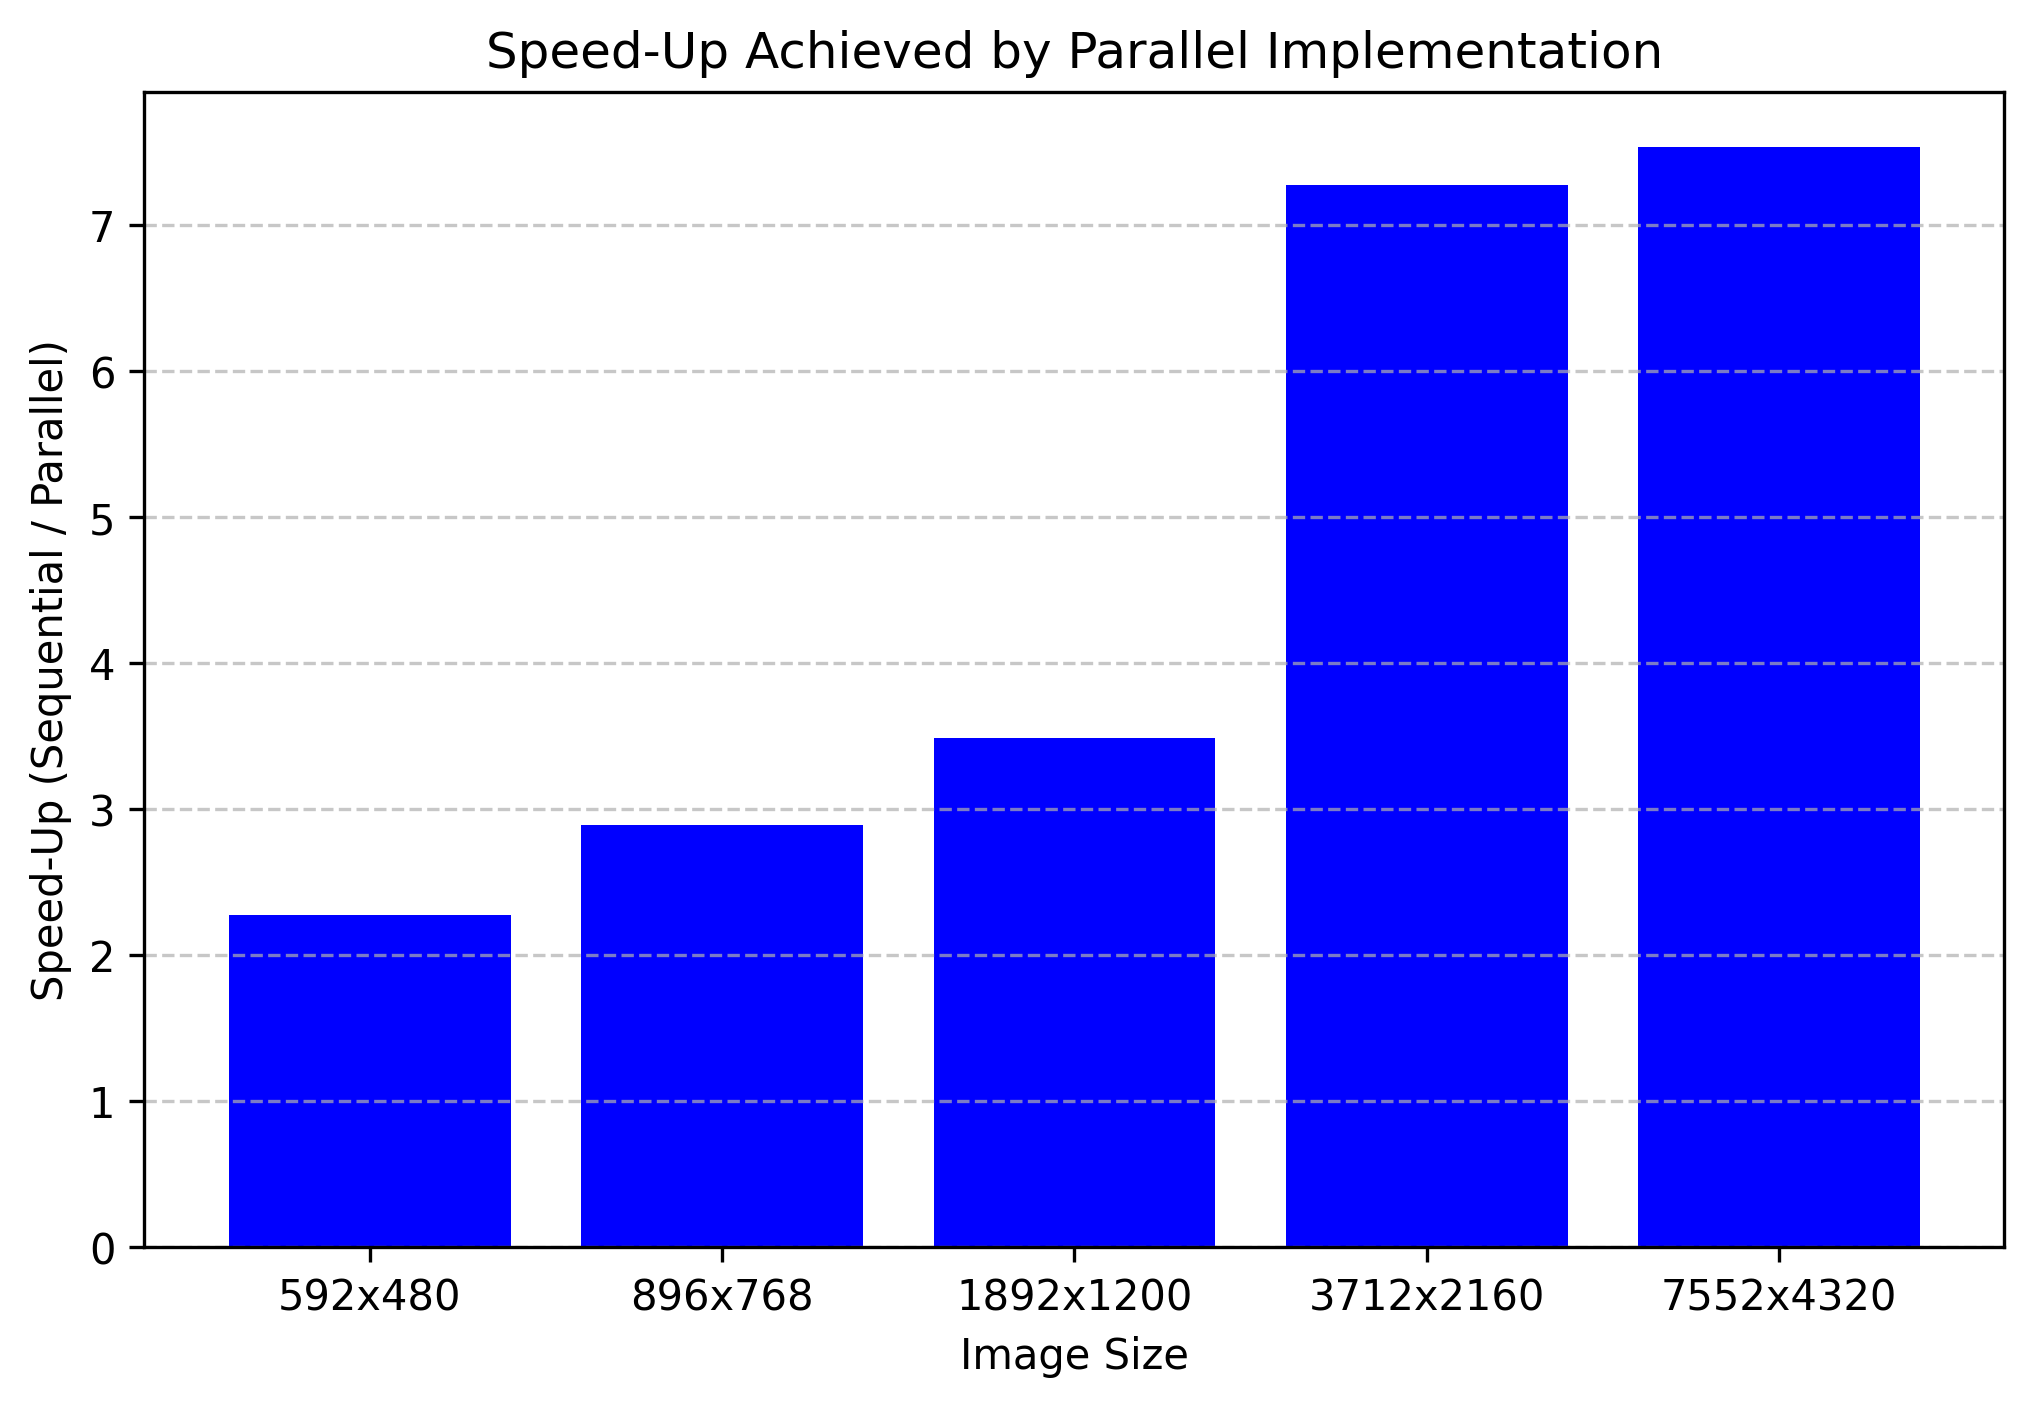
\includegraphics[width=1\columnwidth]{speedup.png}
    \caption{Speed-up achieved by the parallel implementation for different image sizes.}
    \label{fig:speedup}
\end{figure}

\subsection{Comparison of Configurations}
For smaller images (592x480 and 896x768), increasing the number of threads beyond the number of cores (hyper-threading) resulted in degraded performance due to increased overhead. For larger images (1892x1200, 3712x2160, and 7552x4320), hyper-threading provided marginal improvements in some cases but often led to performance degradation due to resource contention. The best performance was consistently achieved with a number of threads equal to the number of cores.

\subsection{Failure Cases and Improvements}
For smaller images, the parallel implementation did not provide significant speed-up due to the overhead of parallelization. Additionally, for very large images (7552x4320), the performance degraded when using more than 8 cores, likely due to increased communication overhead between threads. Future work could focus on optimizing the parallel algorithm for smaller images and reducing the overhead for large images by improving load balancing.

\section{Conclusion}

The parallelized seam carving algorithm achieved significant speed-up for large images, with the best performance observed using 4 to 8 cores. However, for smaller images, the overhead of parallelization outweighed the benefits. Hyper-threading provided limited improvements and often degraded performance due to resource contention. Future work could focus on optimizing the algorithm for smaller images and further reducing the overhead for large images.

\bibliographystyle{IEEEtran}
\bibliography{bibliography}

\end{document}